\textbf{Atmasiddha, Prachi (IISER); Bein, Samuel (Florida State U.)}\\
We present the results of the synchronization of the MA5
implementation of the SUS-14-001 ``top tagging" SUSY search for top squarks.  The
performance of the implementation is evaluated by comparing the
MA5-derived results with a set of cut flow tables and kinematic
distributions provided by CMS for this purpose. The simplified model
T2tt (Fig. \ref{fig:T2tt}) is used as a common benchmark, with values of the masses of the
stop and neutralino taking on a range of values. Two types of
comparisons are given in 
Figs. \ref{table:T2tt-500-125}-\ref{table:T2tt-650-50}: cut flow tables and normalized
kinematic distributions. In some cases the
cut flow tables give the number of events normalized to 100\%; in
other cases the tables are normalized to the cross section times the
integrated luminosity. The normalization convention used by CMS was
followed. Question marks hold the place of values that were not
provided in the CMS cut flow tables.
%%%%%%%%%%%%%%%%%%%%%%%%%%%%%%%%%%%%%%%%%%%%%%%%%
   \begin{figure}
  \centering
    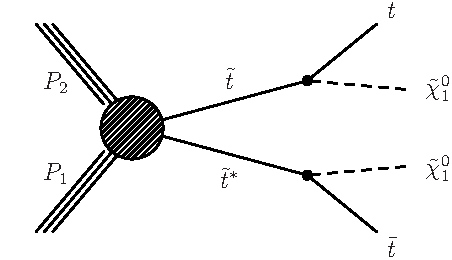
\includegraphics[width=0.5\textwidth]{figures/Appendices/Ma5ValidationSUS13012/T2tt.pdf}
      \caption{Diagram for the T2tt SMS topology. Several mass
        combinations of the stop and LSP are used in the tables below
        as benchmark comparison scenarios.}
      \label{fig:T2tt}
\end{figure}

\begin{table}
    \begin{centering}
    \begin{tabular}{  c | c | c  }
    \hline
    Cut Name & CMS Count(Eff) & MA5 Count(Eff)\\
    \hline
        Event Cleaning & 98.13 (xxx) & 98.13 (xxx)\\
    No Mu & 72.16 (73\%) & 72.21 (73\%)\\
    No Ele & 55.41 (76\%) & 55.50 (76\%)\\
    Njet70$>$1 & 49.55 (89\%) & 50.07 (90\%)\\
    Njet50$>$3 & 31.16 (62\%) & 32.14 (64\%)\\
    Njet30$>$4 & 26.25 (84\%) & 27.10 (84\%)\\
    Min $\Delta(\phi)$ & 22.46 (85\%) & 23.15 (85\%)\\
    Nbjets$>$0 & 19.63 (87\%) & 19.69 (85\%)\\
    MET$>$200 & 12.21 (62\%) & 12.95 (65\%)\\
    Top Reco & - (-) & 5.79 (44\%)\\
    MTsum$>$500 & 4.87 (39\%) & 4.95 (85\%)\\
\hline
    \end{tabular}
    \caption{The acceptance cut flow for the baseline selection in CMS SUS-14-001 for
    model point T2tt-500-125 and the MA5 results are given in column 3.}
    \label{table:T2tt-500-125}
    \end{centering}
    \end{table}

    \begin{table}
    \begin{centering}
    \begin{tabular}{  l | c | c  }
    \hline
    Signal Region Name & CMS & MA5\\
    \hline
    MET200-350,  Nbjets=1 & 1.19 & 1.25\\ 
 \hline 
MET$>$350,  Nbjets=1 & 0.93 & 1.12\\ 
 \hline 
MET200-350,  Nbjets$>$1 & 1.64 & 1.38\\ 
 \hline 
MET$>$350,  Nbjets$>$1 & 1.11 & 1.19\\ 
 \hline 
\hline
    \end{tabular}
    \caption{The signal region (SR) counts in CMS CMS-SUS-14-001 for
    the signal model working pointT2tt-500-125 after all selection has been applied. Column 2 is the CMS account,
    and our own results displayed in column 3. These counts were determined by applying the SR selection to the end of the cut flow featured in table \ref{table:T2tt-500-125}.}
    \end{centering}
    \end{table}



\begin{table}
    \begin{centering}
    \begin{tabular}{  c | c | c  }
    \hline
    Cut Name & CMS Count(Eff) & MA5 Count(Eff)\\
    \hline
        Event Cleaning & 97.44 (xxx) & 97.44 (xxx)\\
    No Mu & 72.5 (74\%) & 71.81 (73\%)\\
    No Ele & 55.55 (76\%) & 54.98 (76\%)\\
    Njet70$>$1 & 52.72 (94\%) & 51.86 (94\%)\\
    Njet50$>$3 & 34.55 (65\%) & 34.66 (66\%)\\
    Njet30$>$4 & 28.49 (82\%) & 28.86 (83\%)\\
    Min $\Delta(\phi)$ & 24.98 (87\%) & 25.22 (87\%)\\
    Nbjets$>$0 & 21.81 (87\%) & 21.67 (85\%)\\
    MET$>$200 & 17.6 (80\%) & 17.73 (81\%)\\
    Top Reco & - (-) & 9.10 (51\%)\\
    MTsum$>$500 & 8.37 (47\%) & 8.52 (93\%)\\
\hline
    \end{tabular}
    \caption{The acceptance cut flow for the baseline selection in CMS SUS-14-001 for
    model point T2tt-650-25 and the MA5 results are given in column 3.}
    \label{table:T2tt-650-25}
    \end{centering}
    \end{table}

    \begin{table}
    \begin{centering}
    \begin{tabular}{  l | c | c  }
    \hline
    Signal Region Name & CMS & MA5\\
    \hline
    MET200-350,  Nbjets=1 & 1.06 & 0.91\\ 
 \hline 
MET$>$350,  Nbjets=1 & 2.49 & 2.93\\ 
 \hline 
MET200-350,  Nbjets$>$1 & 1.34 & 1.24\\ 
 \hline 
MET$>$350,  Nbjets$>$1 & 3.48 & 3.43\\ 
 \hline 
\hline
    \end{tabular}
    \caption{The signal region (SR) counts in CMS CMS-SUS-14-001 for
    the signal model working pointT2tt-650-25 after all selection has been applied. Column 2 is the CMS account,
    and our own results displayed in column 3. These counts were determined by applying the SR selection to the end of the cut flow featured in table \ref{table:T2tt-650-25}.}
    \end{centering}
    \end{table}


\begin{table}
    \begin{centering}
    \begin{tabular}{  c | c | c  }
    \hline
    Cut Name & CMS Count(Eff) & MA5 Count(Eff)\\
    \hline
        Event Cleaning & 15662.0 (xxx) & 15662.0 (xxx)\\
    No Mu & - (-) & 11568.97 (73\%)\\
    No Ele & 8802.0 (56\%) & 8927.82 (77\%)\\
    Njet70$>$1 & - (-) & 7380.74 (82\%)\\
    Njet50$>$3 & - (-) & 4350.13 (58\%)\\
    Njet30$>$4 & 3113.0 (35\%) & 3653.80 (83\%)\\
    Min $\Delta(\phi)$ & 2205.0 (70\%) & 2972.08 (81\%)\\
    Nbjets$>$0 & 2200.0 (99\%) & 2539.64 (85\%)\\
    MET$>$200 & - (-) & 1010.90 (39\%)\\
    Top Reco & - (-) & 314.46 (31\%)\\
    MTsum$>$500 & 182.9 (8\%) & 213.18 (67\%)\\
\hline
    \end{tabular}
    \caption{The acceptance cut flow for the baseline selection in CMS SUS-14-001 for
    model point T2tt-350-0 and the MA5 results are given in column 3.}
    \label{table:T2tt-350-0}
    \end{centering}
    \end{table}

    \begin{table}
    \begin{centering}
    \begin{tabular}{  l | c | c  }
    \hline
    Signal Region Name & CMS & MA5\\
    \hline
    MET200-350,  Nbjets=1 & - & 95.08\\ 
 \hline 
MET$>$350,  Nbjets=1 & - & 13.66\\ 
 \hline 
MET200-350,  Nbjets$>$1 & - & 90.88\\ 
 \hline 
MET$>$350,  Nbjets$>$1 & 7.5 & 13.55\\ 
 \hline 
\hline
    \end{tabular}
    \caption{The signal region (SR) counts in CMS CMS-SUS-14-001 for
    the signal model working pointT2tt-350-0 after all selection has been applied. Column 2 is the CMS account,
    and our own results displayed in column 3. These counts were determined by applying the SR selection to the end of the cut flow featured in table \ref{table:T2tt-350-0}.}
    \end{centering}
    \end{table}
    
   \begin{figure}
  \caption{MA5 and CMS unit-normalized kinematic distributions after the baseline
    selection for the T2tt working point (350,0).}
  \centering
    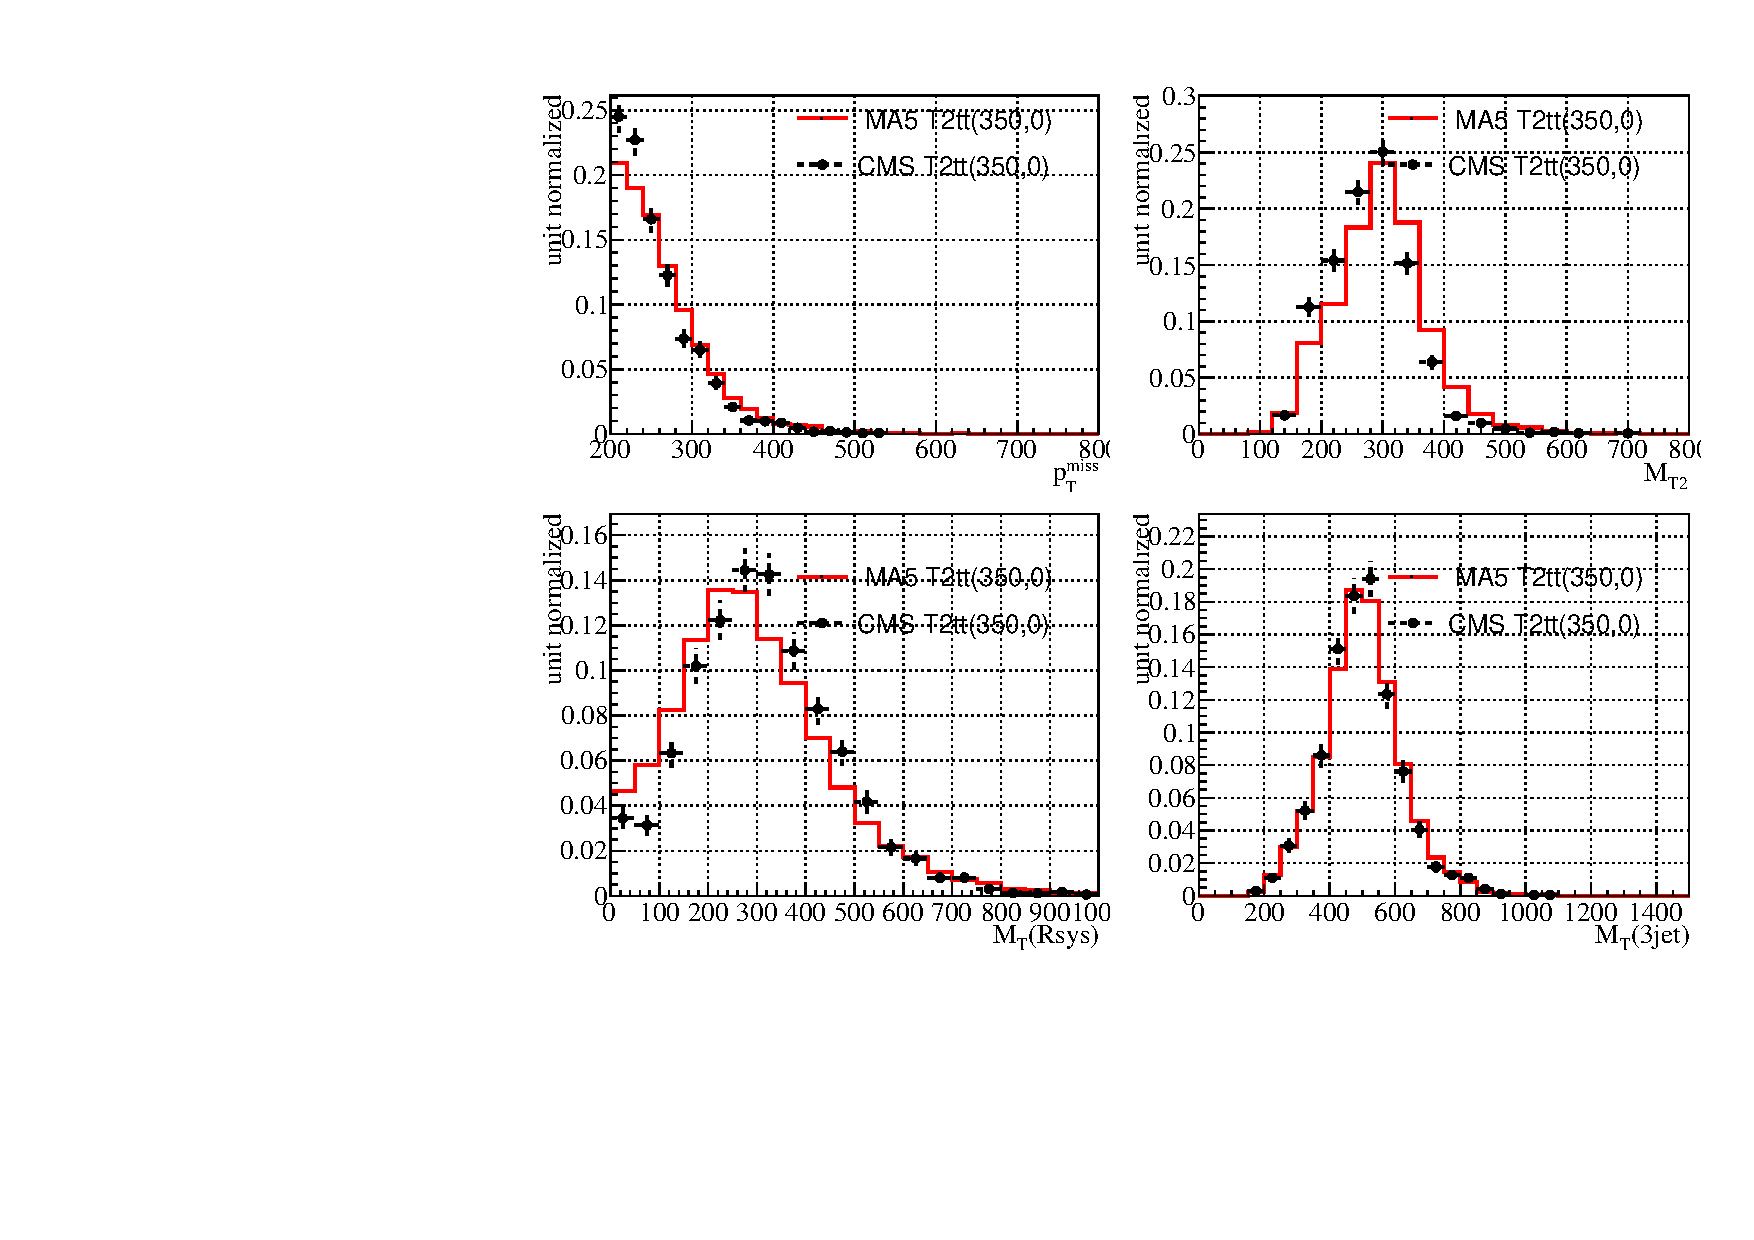
\includegraphics[width=\textwidth]{figures/Appendices/Ma5ValidationSUS13012/T2tt-350-0.pdf}
\end{figure}



\begin{table}
    \begin{centering}
    \begin{tabular}{  c | c | c  }
    \hline
    \hline
    Cut Name & CMS Count(Eff) & MA5 Count(Eff)\\
    \hline
        Event Cleaning & 1660.0 (xxx) & 1660.0 (xxx)\\
    No Mu & - (-) & 1229.14 (74\%)\\
    No Ele & 927.0 (55\%) & 942.80 (76\%)\\
    Njet70$>$1 & - (-) & 856.80 (90\%)\\
    Njet50$>$3 & - (-) & 551.71 (64\%)\\
    Njet30$>$4 & 419.0 (45\%) & 468.27 (84\%)\\
    Min $\Delta(\phi)$ & 360.0 (85\%) & 400.29 (85\%)\\
    Nbjets$>$0 & 314.0 (87\%) & 341.67 (85\%)\\
    MET$>$200 & - (-) & 229.78 (67\%)\\
    Top Reco & - (-) & 105.02 (45\%)\\
    MTsum$>$500 & 85.9 (27\%) & 90.82 (86\%)\\
\hline
    \hline
    \end{tabular}
    \caption{The acceptance cut flow for the baseline selection in CMS SUS-14-001 for
    model point T2tt-500-100 and the MA5 results are given in column 3.}
    \label{table:T2tt-500-100}
    \end{centering}
    \end{table}

    \begin{table}
    \begin{centering}
    \begin{tabular}{  l | c | c  }
    \hline
        \hline
    Signal Region Name & CMS & MA5\\
    \hline
    MET200-350,  Nbjets=1 & - & 21.48\\ 
 \hline 
MET$>$350,  Nbjets=1 & - & 20.52\\ 
 \hline 
MET200-350,  Nbjets$>$1 & - & 25.31\\ 
 \hline 
MET$>$350,  Nbjets$>$1 & 19.8 & 23.50\\ 
 \hline 
\hline
    \end{tabular}
    \caption{The signal region (SR) counts in CMS CMS-SUS-14-001 for
    the signal model working pointT2tt-500-100 after all selection has been applied. Column 2 is the CMS account,
    and our own results displayed in column 3. These counts were determined by applying the SR selection to the end of the cut flow featured in table \ref{table:T2tt-500-100}.}
    \end{centering}
    \end{table}
    
   \begin{figure}
  \caption{MA5 and CMS unit-normalized kinematic distributions after the baseline
    selection for the T2tt working point (500,100).}
  \centering
    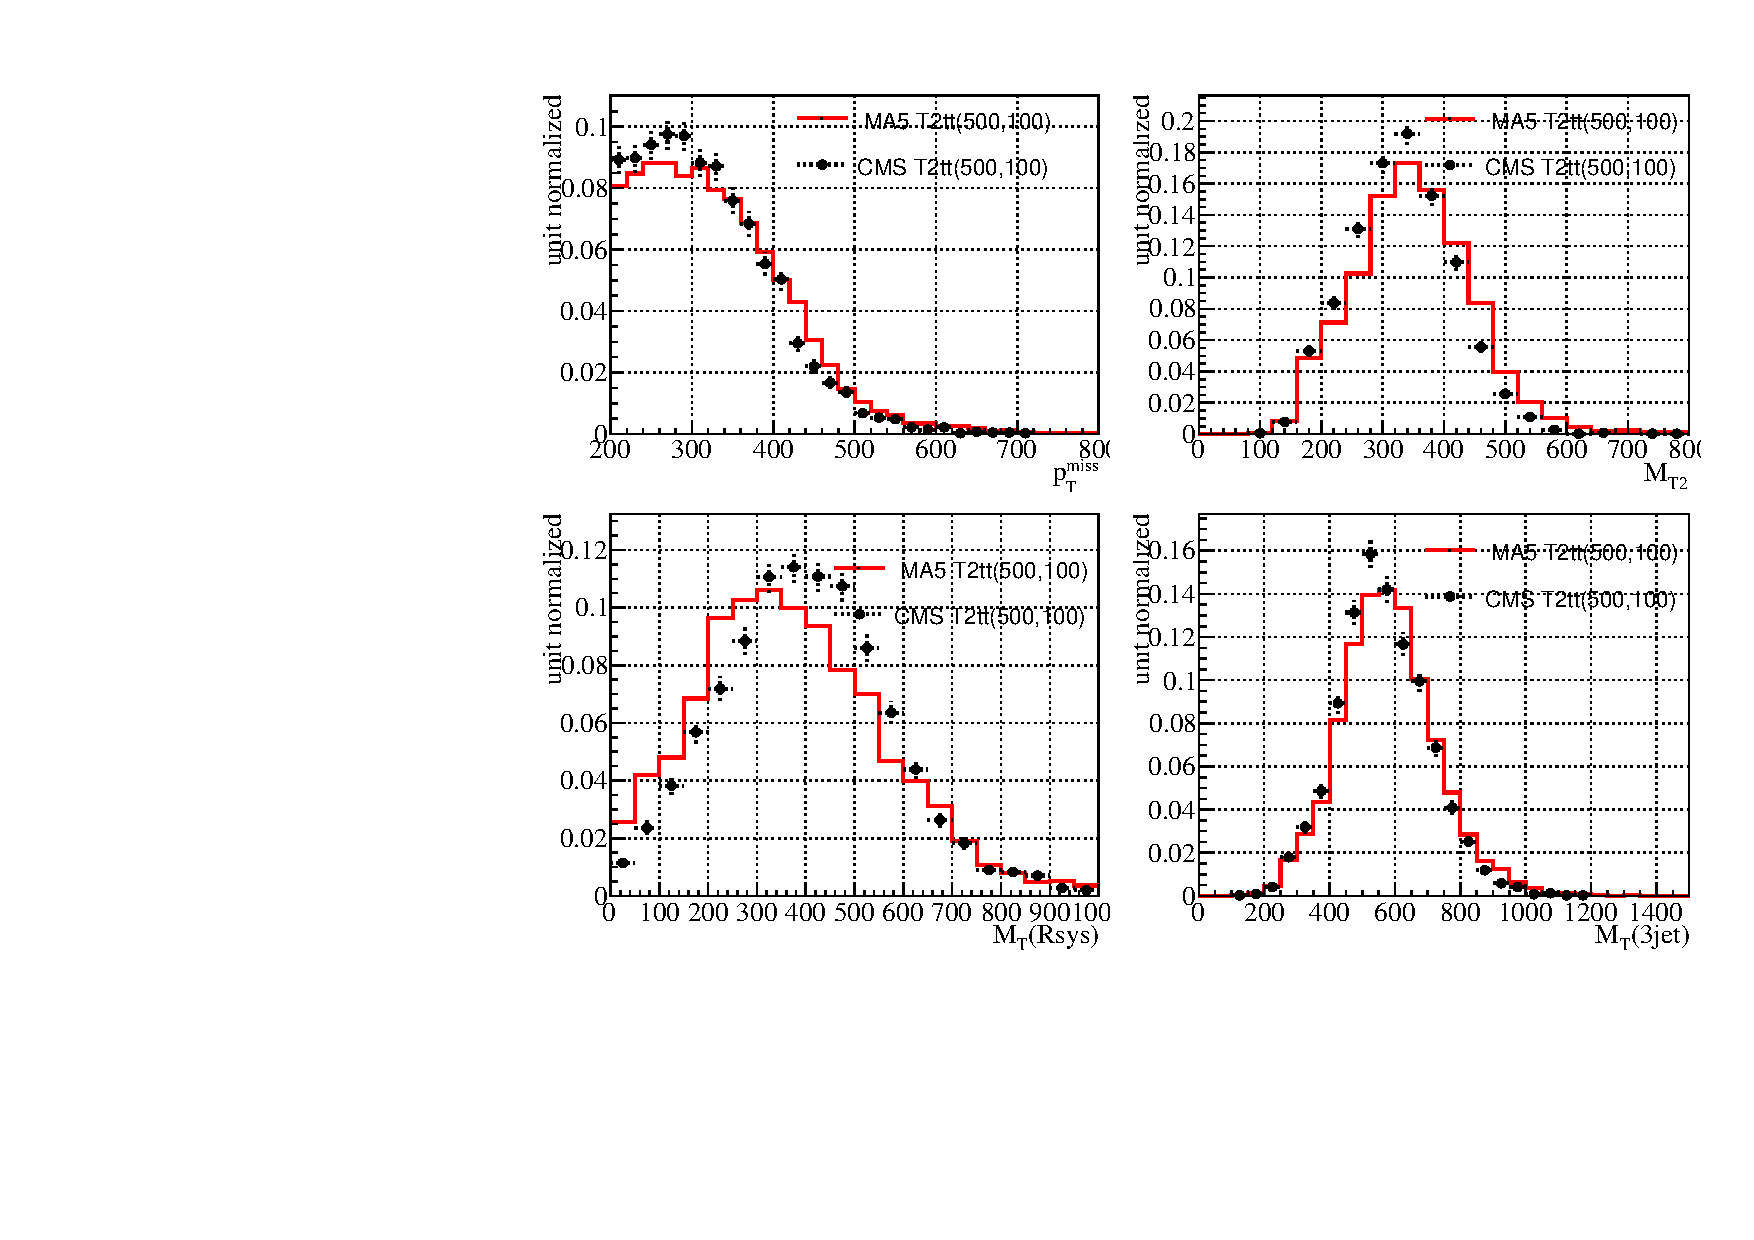
\includegraphics[width=\textwidth]{figures/Appendices/Ma5ValidationSUS13012/T2tt-500-100.pdf}
\end{figure}


\begin{table}
    \begin{centering}
    \begin{tabular}{  c | c | c  }
    \hline
        \hline
    Cut Name & CMS Count(Eff) & MA5 Count(Eff)\\
    \hline
        Event Cleaning & 270.8 (xxx) & 270.8 (xxx)\\
    No Mu & - (-) & 199.25 (73\%)\\
    No Ele & 152.0 (56\%) & 152.26 (76\%)\\
    Njet70$>$1 & - (-) & 143.65 (94\%)\\
    Njet50$>$3 & - (-) & 95.87 (66\%)\\
    Njet30$>$4 & 75.0 (49\%) & 79.95 (83\%)\\
    Min $\Delta(\phi)$ & 66.0 (88\%) & 69.84 (87\%)\\
    Nbjets$>$0 & 58.0 (87\%) & 59.99 (85\%)\\
    MET$>$200 & - (-) & 48.58 (80\%)\\
    Top Reco & - (-) & 25.36 (52\%)\\
    MTsum$>$500 & 22.7 (39\%) & 23.71 (93\%)\\
\hline
    \end{tabular}
    \caption{The acceptance cut flow for the baseline selection in CMS SUS-14-001 for
    model point T2tt-650-50 and the MA5 results are given in column 3.}
    \label{table:T2tt-650-50}
    \end{centering}
    \end{table}

    \begin{table}
    \begin{centering}
    \begin{tabular}{  l | c | c  }
    \hline
    Signal Region Name & CMS & MA5\\
    \hline
    MET200-350,  Nbjets=1 & - & 2.77\\ 
 \hline 
MET$>$350,  Nbjets=1 & - & 8.08\\ 
 \hline 
MET200-350,  Nbjets$>$1 & - & 3.35\\ 
 \hline 
MET$>$350,  Nbjets$>$1 & 9.3 & 9.49\\ 
 \hline 
\hline
    \end{tabular}
    \caption{The signal region (SR) counts in CMS CMS-SUS-14-001 for
    the signal model working pointT2tt-650-50 after all selection has been applied. Column 2 is the CMS account,
    and our own results displayed in column 3. These counts were determined by applying the SR selection to the end of the cut flow featured in table \ref{table:T2tt-650-50}.}
    \end{centering}
    \end{table}


   \begin{figure}
  \caption{MA5 and CMS unit-normalized kinematic distributions after the baseline
    selection for the T2tt working point (650,50).}
  \centering
    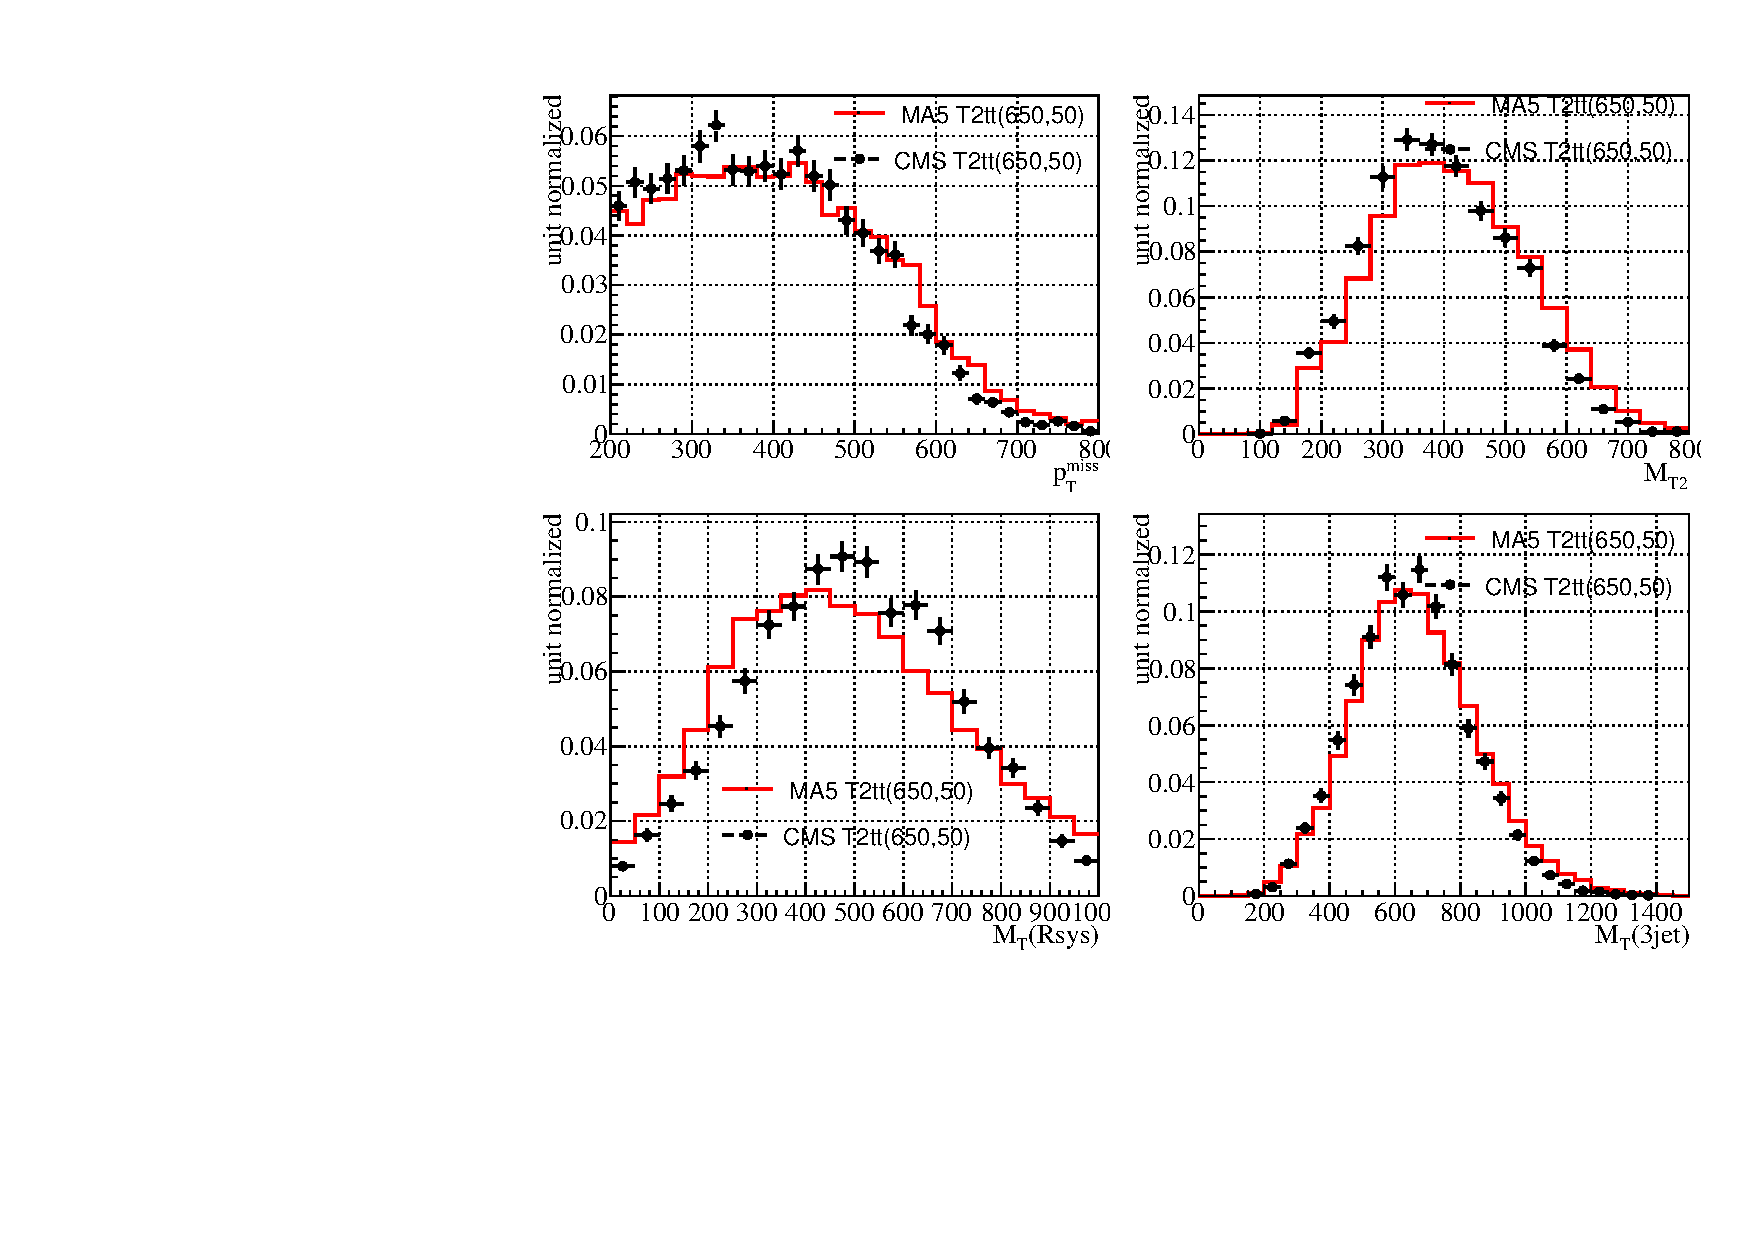
\includegraphics[width=\textwidth]{figures/Appendices/Ma5ValidationSUS13012/T2tt-650-50.pdf}
\end{figure}

%%%%%%%%%%%%%%%%%%%%%%%%%%%%%%%%%%%%%%%%%%%%%%%%%
